\chapter{Experimental Evaluation and Discussion}
\label{chap:evaluation}

This chapter evaluates the closed-loop stacks defined in
Chapter~\ref{chap:control}. The assessment has two parts.
Sections~\ref{sec:eval:tracking}--\ref{sec:eval:robustness} compare the matched
stacks \ppoROM{} and \ppoIDFD{}, which differ only in the actuator
representation. Section~\ref{sec:eval:adaptation} examines online adaptation
inside \ppoAAMFD{}, where the action contract is different and only within-stack
comparisons are valid. Section~\ref{sec:eval:discussion} draws the two parts
together.

The first part concerns tracking, command behaviour, response time, and
robustness under the reserved plant configurations. The second part concerns
whether a history-conditioned residual improves on a frozen base when cutter
mass changes during the episode.

\section{Experimental Protocol}
\label{sec:eval:hypotheses}

\subsection{Test Conditions and Comparisons}
\label{sec:eval:matrix}

All closed-loop results use held-out terrain meshes, eleven trajectory families,
a truck speed of \unit[4]{km/h}, a \unit[26]{m} scoring window, and sixteen
reserved plant configurations. The matched comparison is between \ppoROM{} and
\ppoIDFD{}. These stacks share the training configuration and differ in the
actuator representation. Adaptation is assessed only inside \ppoAAMFD{}, by
comparing a frozen base policy, a capacity-matched residual without history,
and a history-conditioned residual.

The results are paired by environment or by mesh and trajectory family. Error
metrics are reported separately for lateral tracking and cut height because the
two errors describe different aspects of the task. Confidence intervals are
obtained by paired bootstrap. Checkpoints are selected using the validation or
training criterion specified for each experiment and are then evaluated once on
the held-out set.

\subsection{Comparative Scope and Scoring}
\label{sec:eval:standing}

\ppoROM{} and \ppoIDFD{} form the cross-stack comparison. \ppoAAMFD{} has a
different action contract and is therefore not ranked against that pair. Its
results are interpreted only through within-stack comparisons.

\subsection{Scoring Horizon}
\label{sec:eval:horizon}

All reported closed-loop results use the full \unit[26]{m} trajectory rather
than a shorter selection window.

\section{Closed-Loop Task Performance}
\label{sec:eval:tracking}

The first comparison reports closed-loop tracking of \ppoROM{} and \ppoIDFD{}
on the held-out meshes and trajectory families.

The task is scored on two independent error channels, drawn side by side in
Figure~\ref{fig:eval:paths}: lateral error is deviation from the planned
cutting line in the horizontal plane, and cut-height error is deviation from the
intended vertical cut. They are kept separate throughout because a controller
can improve one while worsening the other. Ground contact, impacts and tool
acceleration are reported alongside them as checks on motion quality.

\begin{figure}[tbp]
  \centering
  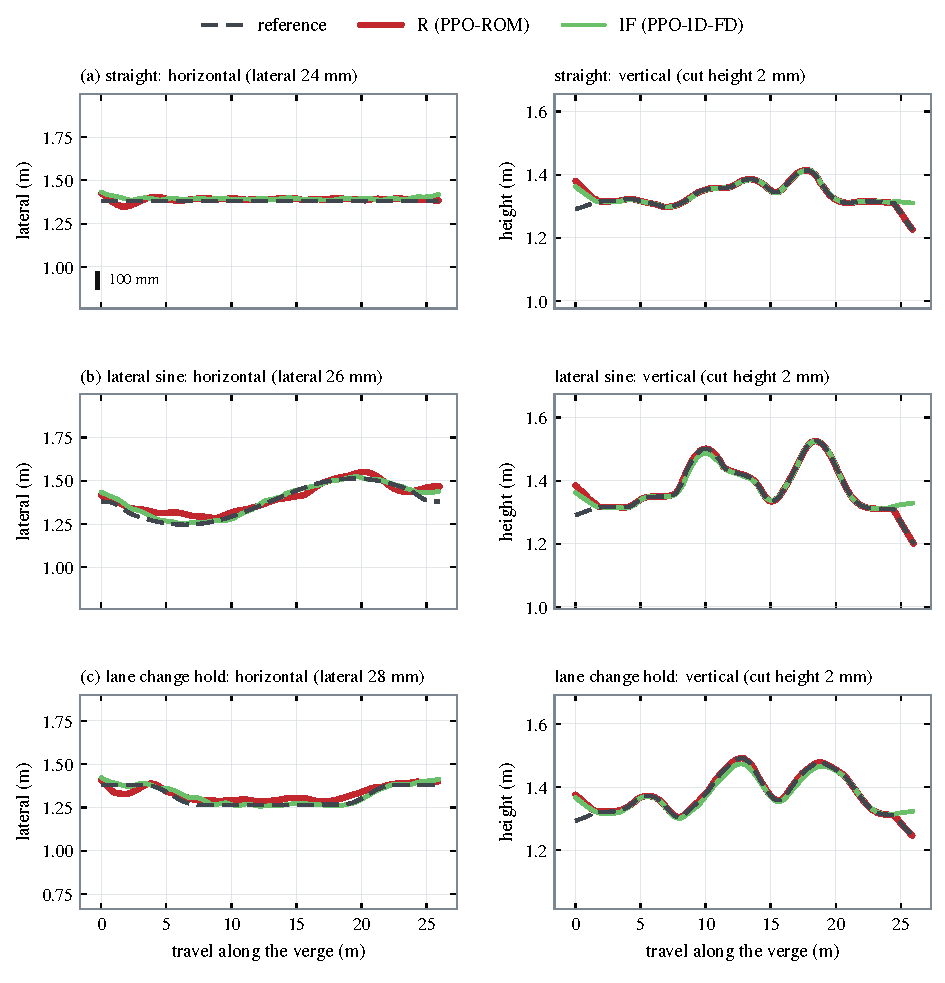
\includegraphics[width=\textwidth]{images/ch7/ch7_e1_paths}
  \caption{Cutter path against the reference on held-out mesh $1337$, for three
  structurally different trajectory families: a flat line, a smooth periodic
  sweep and a step-and-hold. The left column is the horizontal plane and the
  right column the vertical plane over the same drive. The vertical reference is
  not recorded directly and is recovered as
  $z_{\mathrm{ref}} = z_{\mathrm{cutter}} - e_{\mathrm{cut}}$, so both columns
  compare reference against actual. In the vertical panels the reference is
  largely hidden beneath both traces, which is what a millimetre-scale
  cut-height error looks like drawn at path scale.}
  \label{fig:eval:paths}
\end{figure}

Table~\ref{tab:eval:tracking} compares the matched pair over $33$ held-out
(mesh, family) conditions. Median errors are low for both stacks, and the p95
values move in the same direction as the means, so the improvement also reduces
the larger tracking deviations rather than only the average.

\begin{table}[tbp]
  \centering
  \caption{Closed-loop performance over $33$ paired held-out conditions. The
  matched stacks differ only in the actuator representation.}
  \label{tab:eval:tracking}
  \begin{tabular}{lcc}
    \toprule
    & \ppoROM{} & \ppoIDFD{} \\
    \midrule
    lateral error, mean (m) & $0.1026$ & $\mathbf{0.0703}$ \\
    lateral error, median (m) & $0.0392$ & $\mathbf{0.0281}$ \\
    lateral error, p95 (m) & $0.4664$ & $\mathbf{0.2665}$ \\
    cut-height error, mean (m) & $0.0084$ & $\mathbf{0.0063}$ \\
    cut-height error, median (m) & $\mathbf{0.0013}$ & $0.0031$ \\
    ground contact & $\mathbf{0.9623}$ & $0.9529$ \\
    hard impacts & $0.0947$ & $\mathbf{0.0905}$ \\
    tool acceleration p95 (m/s$^2$) & $39.90$ & $\mathbf{39.02}$ \\
    \bottomrule
  \end{tabular}
\end{table}

\begin{figure}[tbp]
  \centering
  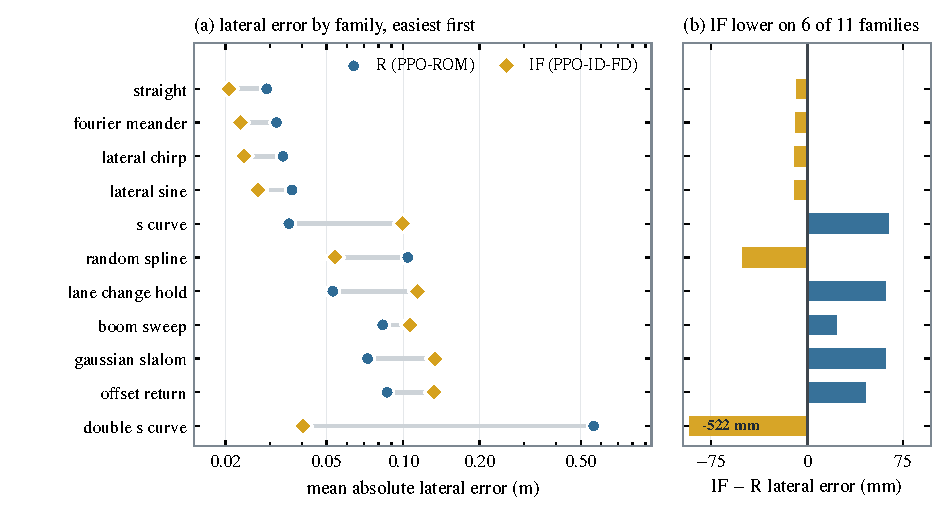
\includegraphics[width=\textwidth]{images/ch7/ch7_e1_tracking}
  \caption{Lateral error by trajectory family for the matched pair. The
  aggregate difference is concentrated in the more difficult families.}
  \label{fig:eval:tracking}
\end{figure}

Figure~\ref{fig:eval:tracking} resolves the aggregate by trajectory family.
\ppoIDFD{} reduces mean lateral error from \unit[0.103]{m} to \unit[0.070]{m}
and mean cut-height error from \unit[8.4]{mm} to \unit[6.3]{mm} over the $33$
paired conditions. The advantage is not uniform: \ppoIDFD{} is better on six of
the eleven families and \ppoROM{} on five, with the largest difference on the
double S-curve. The difference is concentrated on the more demanding families.
Both stacks follow the simpler paths closely.

\section{Actuator Representation and Dynamic Response}
\label{sec:eval:delay}

The same matched pair is now examined in the actuation channel: transport
delay, closed-loop step response, and command effort.

\subsection{Plant Delay and Step Response}
\label{sec:eval:delay-plant}

Open-loop excitation measured a command-to-pressure delay of approximately
\unit[117]{ms}. Cylinder extension and joint motion began at the same time,
which confirms that the dominant delay is hydraulic rather than kinematic. The
similar values across excitation amplitudes indicate that this delay is a stable
property of the simulated actuation chain.

\begin{table}[tbp]
  \centering
  \caption{Transport latency along the actuation chain, in milliseconds.
  Values are medians over open-loop excitation runs at \unit[60]{Hz}.}
  \label{tab:eval:delay}
  \begin{tabular}{lcccc}
    \toprule
    & \multicolumn{4}{c}{excitation amplitude} \\
    \cmidrule(lr){2-5}
    Link & $0.05$ & $0.15$ & $0.35$ & $0.70$ \\
    \midrule
    command $\rightarrow$ differential pressure & $117$ & $117$ & $117$ & $150$ \\
    command $\rightarrow$ cylinder velocity & $183$ & $167$ & $133$ & $117$ \\
    command $\rightarrow$ cylinder extension & $117$ & $117$ & $100$ & $100$ \\
    command $\rightarrow$ joint position & $117$ & $117$ & $100$ & $100$ \\
    \bottomrule
  \end{tabular}
\end{table}

The commanded-step experiment measures the closed-loop response to a
\unit[100]{mm} change in the reference line. Rise time is measured from
$10$ to $90\,\%$ of the step. Settling time is the first point at which the
error remains within \unit[20]{mm} for \unit[0.5]{s}.
\label{sec:eval:step-response}

\begin{table}[tbp]
  \centering
  \caption{Response to a \unit[100]{mm} commanded step. Values are median
  times over sixteen environments.}
  \label{tab:eval:step}
  \begin{tabular}{lcccc}
    \toprule
    Stack & detected response & rise & settled & overshoot \\
    \midrule
    \ppoROM{} & $333$ & $617$ & $2633$ & $57\,\%$ \\
    \ppoIDFD{} & $350$ & $717$ & $2183$ & $73\,\%$ \\
    \bottomrule
  \end{tabular}
  \\[2pt]
  \footnotesize Times are in milliseconds.
\end{table}

\ppoIDFD{} settles about \unit[0.45]{s} earlier, whereas \ppoROM{} has lower
overshoot. The command rate limit alone requires at least \unit[417]{ms} to
complete this step, and both stacks require more than \unit[2]{s} to settle.
Reducing hydraulic delay alone would therefore not remove the observed settling
time; the command rate, the policy response and the reference handling would
have to change with it.

Closed-loop settling is much slower than the hydraulic delay. Command-rate
limits and policy dynamics dominate the response time. The actuator path changes
the shape of the step, not the main settling time.

\subsection{Control Effort}
\label{sec:eval:effort}

\begin{table}[tbp]
  \centering
  \caption{Control effort on a held-out mesh. Lateral error is in millimetres;
  commands are in normalised units.}
  \label{tab:eval:effort}
  \begin{tabular}{lcccc}
    \toprule
    Stack & RMS command & rate RMS & reversals/s & lateral error \\
    \midrule
    \ppoROM{} & $0.586$ & $7.55$ & $40.0$ & $120.1$ \\
    \ppoIDFD{} & $0.827$ & $10.68$ & $\mathbf{10.6}$ & $\mathbf{26.8}$ \\
    \bottomrule
  \end{tabular}
\end{table}

\begin{figure}[tbp]
  \centering
  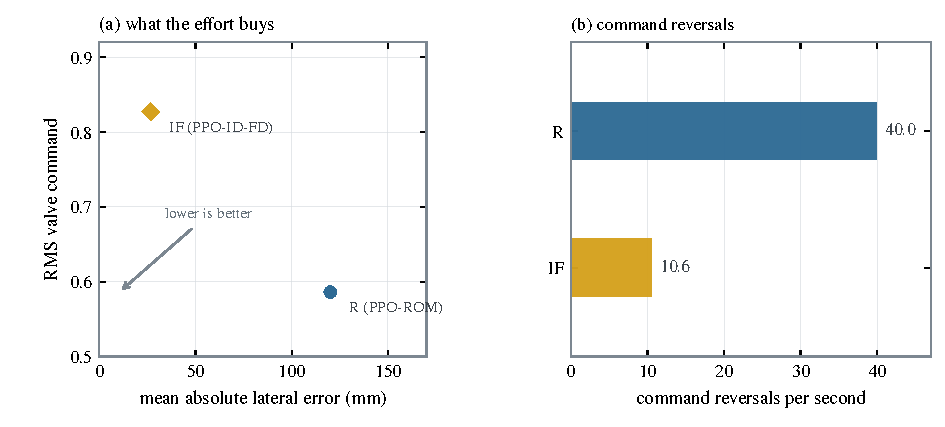
\includegraphics[width=\textwidth]{images/ch7/ch7_control_effort}
  \caption{(a) Control effort against the tracking error it buys for the matched
  pair; the lower left is better. (b) Command reversals per second, which the
  root-mean-square command does not reveal.}
  \label{fig:eval:effort}
\end{figure}

The reversal count identifies rapid changes in command direction that the
root-mean-square magnitude does not reveal, and
Figure~\ref{fig:eval:effort} pairs each stack's effort with the tracking error
it buys. A lower RMS command is not preferable when it comes with frequent
reversals and larger path error.

\ppoROM{} uses a smaller command magnitude but reverses almost four times as
often. \ppoIDFD{} uses more actuation, reverses less, and tracks more closely.
Effort is therefore reported together with the tracking it buys.

\section{Generalisation and Robustness}
\label{sec:eval:robustness}

The preceding sections use the held-out evaluation set. This section records
what that set does and does not establish, and then applies a common authority
reduction to all stacks.

The matched stacks generalise to the held-out meshes, trajectory families, and
reserved plant configurations used in this chapter. The randomisation sweep
showed little change in tracking over the tested mechanical variation. Its
hydraulic interpretation is limited because the inverse and forward plant does
not apply the hydraulic factors, while the reduced-order model constrains them
to its identification range.

The held-out evaluation therefore establishes transfer within the tested
simulation population. It does not establish performance on arbitrary hydraulic
conditions or physical hardware.

\subsection{Delivered Stress}
\label{sec:eval:delivered-stress}

The sweep therefore supports robustness to the tested changes in tool mass and
centre-of-mass height. It does not establish robustness to unbounded hydraulic
variation. A common authority perturbation was used to compare all stacks more
directly. This separates a reduction in realised actuator motion from the
specific randomisation factors used during deployment.

\subsection{Actuator Authority}
\label{sec:eval:boundary-design}

Actuator authority was reduced by scaling the realised actuator displacement:
\begin{equation}
  \label{eq:eval:authority}
  \Delta x^{\text{applied}}_k = \kappa\,\Delta x^{\text{actuator}}_k,
  \qquad \kappa \in (0,1].
\end{equation}

Here, $\kappa=1$ represents nominal authority and smaller values reduce the
motion delivered to the plant. The same perturbation is applied after each
stack's actuator representation, which makes the comparison independent of the
individual factor parameterisations.

\begin{figure}[tbp]
  \centering
  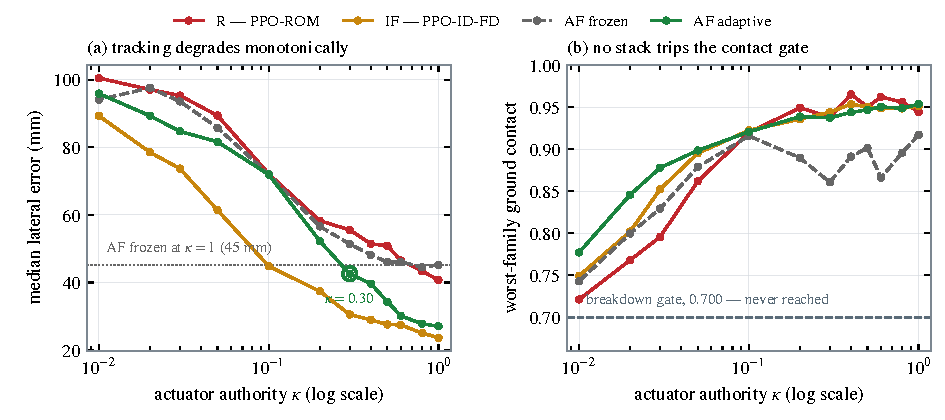
\includegraphics[width=\textwidth]{images/ch7/ch7_kappa_stacks}
  \caption{Lateral tracking and ground contact as actuator authority is reduced.
  The frozen and adaptive arms are compared within \ppoAAMFD{}.}
  \label{fig:eval:kappa-stacks}
\end{figure}

\begin{table}[tbp]
  \centering
  \caption{Authority at which median lateral error first reaches $1.5$ times
  its full-authority value.}
  \label{tab:eval:kappa}
  \begin{tabular}{lccc}
    \toprule
    Stack & nominal error (mm) & threshold (mm) & onset $\kappa$ \\
    \midrule
    \ppoROM{} & $40.69$ & $61.04$ & $0.10$ \\
    \ppoIDFD{} & $23.66$ & $35.49$ & $0.20$ \\
    \ppoAAMFD{} frozen & $45.18$ & $67.78$ & $0.10$ \\
    \ppoAAMFD{} adaptive & $27.03$ & $40.55$ & $0.30$ \\
    \bottomrule
  \end{tabular}
\end{table}

A hard robustness boundary was not observed over the tested authority range,
and \ppoIDFD{} had the lowest lateral error at every rung of the cross-stack
comparison.

No stack reached the contact or safety gate. Within \ppoAAMFD{}, the adaptive
residual holds the frozen residual's nominal lateral error down to
$\kappa=0.30$. This is an authority margin inside \ppoAAMFD{}. It is not a
ranking of \ppoAAMFD{} against \ppoROM{} or \ppoIDFD{}.

\section{Online Adaptation}
\label{sec:eval:adaptation}

The following experiments remain inside \ppoAAMFD{}. They test whether a
residual on the valve command improves on the frozen base when cutter mass
changes during the episode, and how much of any gain depends on live history
and on the size of the plant change.

\subsection{Experiment and Measurement}
\label{sec:eval:instrument}

The online-adaptation experiment changes cutter mass during each episode. The
change time and direction vary across environments. The three compared arms
share the frozen base policy, residual architecture, training budget, and
reward. The base has no residual, the control has a residual with a zeroed
history window, and the adaptive arm receives recent state-action history.

Changing mass during an episode creates a condition that cannot be addressed by
one fixed response. The varying change time prevents the residual from relying
on a fixed event schedule.

Results use $880$ paired environments across five held-out meshes. Lateral and
cut-height effects are evaluated separately. Cut-height effects smaller than
approximately $10\,\%$ are treated as unresolved because of the measurement
resolution; the corresponding lateral threshold is approximately $1.5\,\%$.
The paired design ensures that each arm is assessed under the same terrain,
trajectory, and mass-change condition.

\subsection{Performance Across Seeds}

\begin{table}[tbp]
  \centering
  \caption{History-conditioned residual against the frozen base over five
  training seeds. An asterisk indicates that the paired bootstrap interval
  excludes zero.}
  \label{tab:eval:arms}
  \begin{tabular}{lccc}
    \toprule
    Seed & cut-height gain & lateral gain & interpretation \\
    \midrule
    $17$ & $+39.1\,\%^{*}$ & $+84.9\,\%^{*}$ & improvement \\
    $23$ & $+35.5\,\%^{*}$ & $+4.0\,\%^{*}$ & improvement \\
    $101$ & $+74.7\,\%^{*}$ & $+5.9\,\%^{*}$ & improvement \\
    $42$ & $+43.4\,\%^{*}$ & $-16.1\,\%^{*}$ & trade-off \\
    $7$ & $+4.5\,\%$ & $+55.7\,\%^{*}$ & lateral improvement \\
    \bottomrule
  \end{tabular}
\end{table}

The percentages compare paired environments. A positive value means that the
adaptive arm has lower error than the frozen base for the median paired
environment. The bootstrap marker indicates that the paired difference is
resolved by the stated statistical test.

The adaptive residual improves at least one metric in four of five seeds. No
seed is worse on both metrics. The size of the effect varies, including a
trade-off on seed $42$, which is why the two error channels are not combined.

\subsection{Contribution of History}
\label{sec:eval:attribution}

The capacity-matched control separates the effect of the residual from the
effect of the history it receives.

\begin{table}[tbp]
  \centering
  \caption{Decomposition of the adaptive gain. The control and adaptive arms
  have the same capacity; only the adaptive arm receives live history.}
  \label{tab:eval:control-arm}
  \small
  \begin{tabular}{lcccc}
    \toprule
    & \multicolumn{2}{c}{base $\rightarrow$ control} & \multicolumn{2}{c}{control $\rightarrow$ adaptive} \\
    \cmidrule(lr){2-3}\cmidrule(lr){4-5}
    Seed & cut & lateral & cut & lateral \\
    \midrule
    $17$ & $+63.9\,\%^{*}$ & $-1.2\,\%$ & $-21.1\,\%^{*}$ & $+80.3\,\%^{*}$ \\
    $23$ & $+77.2\,\%^{*}$ & $+42.2\,\%^{*}$ & $-21.2\,\%^{*}$ & $-22.8\,\%^{*}$ \\
    $101$ & $+90.9\,\%^{*}$ & $+56.2\,\%^{*}$ & $-5.2\,\%$ & $-29.9\,\%^{*}$ \\
    $42$ & $+1.3\,\%$ & $-62.2\,\%^{*}$ & $+38.4\,\%^{*}$ & $+124.9\,\%^{*}$ \\
    $7$ & $+95.0\,\%^{*}$ & $+39.7\,\%^{*}$ & $-46.0\,\%^{*}$ & $+12.2\,\%^{*}$ \\
    \bottomrule
  \end{tabular}
\end{table}

This comparison is necessary because a larger residual can improve control even
when it receives no information about the current plant. The control arm has
the same trainable capacity and the same optimisation conditions as the adaptive
arm, so the difference between them is the live history and nothing else.

Residual capacity accounts for most of the cut-height gain in four seeds. The
additional effect of live history is mixed. The control arm is therefore not a
weaker adaptive arm; it isolates history from capacity.

\subsection{Plant-Dependent Contribution}
\label{sec:eval:dose}

To isolate plant-dependent adaptation, the mass-change magnitude was varied and
compared with a sham condition in which the event occurred without a change in
mass. The sham measures the benefit of the residual under the same event
schedule but without plant variation. The lateral benefit beyond the sham
increased with the mass change.

\begin{table}[tbp]
  \centering
  \caption{Lateral gain beyond the sham condition. Every interval excludes
  zero.}
  \label{tab:eval:dose}
  \begin{tabular}{lccc}
    \toprule
    Mass-change magnitude & total gain (mm) & gain beyond sham (mm) & interval (mm) \\
    \midrule
    $1.0$ (sham) & $16.557$ & n/a & n/a \\
    $1.5$ & $20.045$ & $3.796$ & $[2.303, 6.105]$ \\
    $2.0$ & $20.487$ & $3.912$ & $[1.693, 6.415]$ \\
    $2.5$ & $20.490$ & $4.073$ & $[2.318, 6.697]$ \\
    $3.0$ & $23.705$ & $7.410$ & $[4.785, 10.503]$ \\
    \bottomrule
  \end{tabular}
\end{table}

\begin{figure}[tbp]
  \centering
  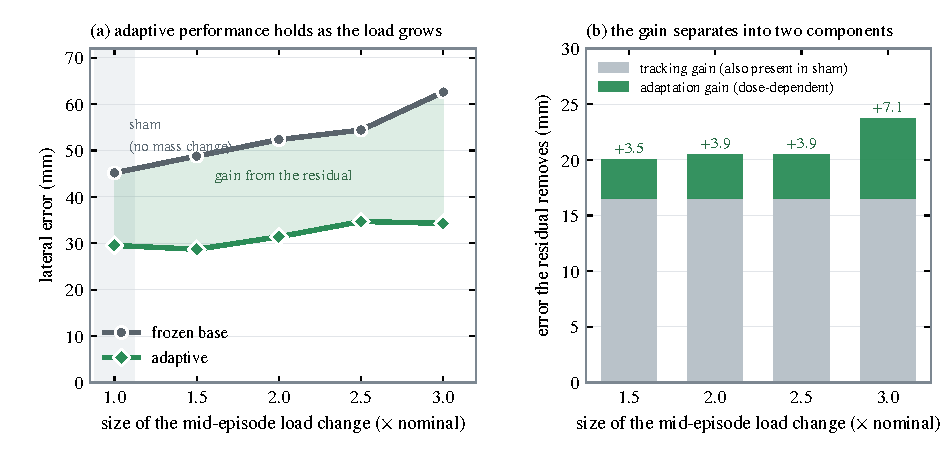
\includegraphics[width=\textwidth]{images/ch7/ch7_dose_response}
  \caption{Lateral performance across mass-change magnitudes. The sham
  condition separates general residual improvement from the contribution that
  increases with the plant change.}
  \label{fig:eval:dose}
\end{figure}

The trend is monotonic and resolved at every tested magnitude. The result is
limited to the perturbation and channel tested here: it does not show that
history conditioning improves every plant change or every task metric, only
that the lateral correction contains a measurable component that scales with
the mass change.

Lateral gain beyond the sham rises from \unit[3.8]{mm} at a $1.5$-fold mass
change to \unit[7.4]{mm} at a $3.0$-fold change. That component is
plant-dependent. It is about $31\,\%$ of the total lateral gain at the largest
change. The cut-height gain does not scale in the same way and is treated as a
general residual effect.

\subsection{The Pressure Channel Through the Load Change}
\label{sec:eval:pressure-signals}

The latent carries mainly seal condition
(Section~\ref{sec:models:aam-content}), and seal condition acts through
pressure, so the pressure the actuator model carries is where any conditioning
should first be visible. Figure~\ref{fig:eval:pressure-stacks} shows it per
cylinder for all three stacks, on the same plant and aligned on the same event.

\begin{figure}[tbp]
  \centering
  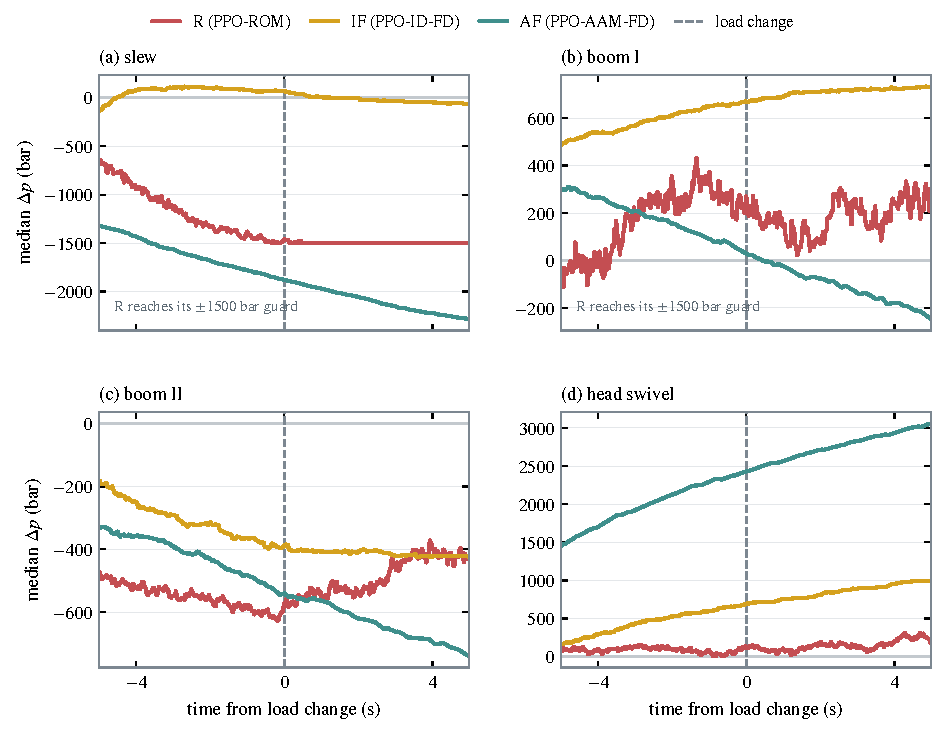
\includegraphics[width=\textwidth]{images/ch7/ch7_pressure_stacks}
  \caption{Median differential pressure per cylinder through the change of load,
  $151$ environments aligned on their own flip instant. The quantity is each
  stack's own actuator-model state, internal to the command ROM for \ppoROM{}
  and the forward model's recursive state for the other two, so the panels show
  what each controller believes about the hydraulics rather than a common
  measurement, and each panel carries its own scale. The slew and boom~I panels
  mark where \ppoROM{} sits on its \unit[1500]{bar} numerical guard.}
  \label{fig:eval:pressure-stacks}
\end{figure}

Two properties of the signal govern how the figure is read. The pressure state
is not a calibrated pressure on any stack: in this window the medians run to
\unit[2295]{bar} and the peaks to \unit[3784]{bar}, which is past what a
cylinder of this size could develop. The rod-force channel carries no supervised
weight and pressure-increment accuracy is only $R^2 = 0.06$ to $0.09$
(Section~\ref{sec:models:rom}). On \ppoROM{} the excursions are additionally
clipped by the \unit[1500]{bar} numerical guard, which binds on the slew and
the first boom cylinder and not on the other two. There is therefore no common
physical level the panels can be read against, and each cylinder is drawn on its
own scale. What the figure supports is the shape of the response either side of
the change, not the level.

Read that way, the traces are consistent with
Section~\ref{sec:eval:attribution}. Pressure state moves at the load change on
every stack, so the residual has access to a channel that reacts to the event.
The adaptive advantage is already present before the event, which is consistent
with continuous conditioning rather than a one-shot transient correction.

\section{Integrated Discussion}
\label{sec:eval:discussion}

\subsection*{Actuator Representation}

The inverse and forward actuator representation improved average tracking in
the matched comparison. It also reduced command reversals substantially.
Although the hydraulic transport delay was short, both stacks responded to a
reference step on a much longer time scale. Command limits and policy dynamics,
rather than the hydraulic delay, dominated closed-loop settling.

The tested stacks transferred to held-out terrain, trajectories, and plant
configurations. The authority experiment showed graceful degradation but did
not identify a hard safety boundary. Within \ppoAAMFD{}, the history-conditioned
residual retained the frozen residual's nominal tracking at lower actuator
authority. This is an authority-margin result, not evidence that it is the best
cross-stack controller.

\subsection*{Online Adaptation}

The history-conditioned residual improved on the frozen base in most training
seeds. The capacity-matched comparison shows that residual capacity explains a
large part of this result, so the overall gain cannot be assigned to history
alone. However, the sham-controlled dose experiment provides direct evidence
of a plant-dependent lateral contribution: the benefit increased with the size
of the mass change.

Online adaptation is therefore supported for the lateral channel under the
tested mass changes. Its contribution depends on plant variation reaching a
channel that the correction can influence and on the correction retaining
usable command authority. These conditions define the scope of the result.

\subsection*{Scope}

History-conditioned control has to be separated from added residual capacity. A
sham-controlled change is required to distinguish a general improvement from a
response that scales with the plant. For this manipulator, the measurable
plant-dependent benefit is limited to lateral tracking under the tested load
changes.
